En este trabajo se obtuvo un diseño preliminar de la geometría de los  sistemas
de intercambio de gases del Motor Rotativo de Combustión a Volumen
Constante~\parencite{toth}, con el objetivo de maximizar la eficiencia del
sistema en un rango de velocidades del motor.
%

El MRCVC es un proyecto que surgió en la Universidad Nacional del Comahue,
inventado y patentado por Jorge Toth~\parencite{toth} en el año 2004, este
proyecto nace en el marco del \emph{Proyecto de Investigación Desarrollo de
modelos y herramientas para la simulación de problemas complejos en ingeniería
mediante fluido dinámica computacional (04/I-251)} y actualmente se encuentra
en etapa de desarrollo.

\begin{figure}
    \centering
    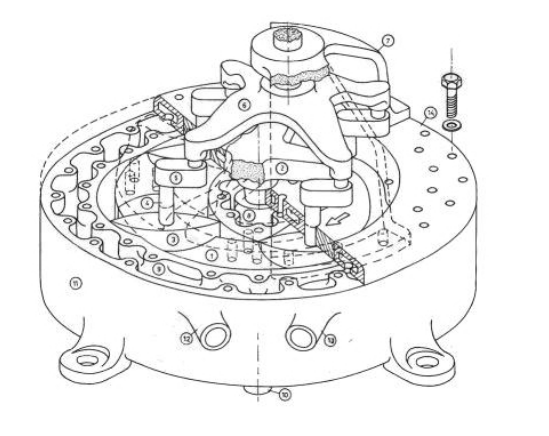
\includegraphics[width=0.5\textwidth]{perspectiva_mrcvc.png}
    \caption{Motor Rotativo de Combustión a Volumen Constante}\label{fig:mrcvc}
\end{figure}

En trabajos anteriores~\parencite{lopez16}\parencite{lopez13}\parencite{roldan}
se han mencionado las características que hacen al MRCVC un motor atractivo, la
geometría de la cámara de combustión y del conjunto rotante permiten que gran
parte del proceso de combustión se realice a volumen constante, además de tener
un balanceo mecánico de fuerzas.
%
Esto permite un funcionamiento más suave del motor, además de una reducción del
ruido y desgaste en comparación a motores rotativos tradicionales (Wankel) y
alternativos.
%
Por otro lado hay que mencionar que los motores rotativos traen consigo una
serie de problemas como la necesidad de introducir aceite a la cámara de
combustión para lubricar elementos móviles, el solape de cámaras durante la
apertura de los puertos y en particular al MRCVC un complejo sistema de
sellos~\parencite{roldan}.

%%%%%%%%%%%%%%%%%%%%%%%%%%%%%%%%%%%%%%%%%%%%%%%%%%%

La motivación de este trabajo surge del deseo de continuar con el
desarrollo del MRCVC, en particular mejorar el pre diseño de los sistemas de
intercambio de gases, sentando la base para una futura optimización de los
mismos en un motor con requisitos de diseño concretos.

%%%%%%%%%%%%%%%%%%%%%%%%%%%%%%%%%%%%%%%%%%%%%%%%%%%
El objetivo de este trabajo es obtener un prediseño satisfactorio
del sistema de intercambio de gases del MRCVC, en particular de la geometría de
los puertos de admisión y escape.
%
El prediseño consiste en definir las métricas a utilizar para medir la
eficiencia del sistema, así como también poder comparar cualitativamente y
cuantitativamente diferentes geometrías.

Debido al costo computacional de las simulaciones necesarias para realizar esta
optimización, se restringe el modelado de la geometría a definir posiciones
angulares y diámetros, no se repara en detalles como la forma de la transición
entre las paredes del puerto hacia la cámara de combustión, el ángulo del puerto
respecto al estator, etc.

%%%%%%%%%%%%%%%%%%%%%%%%%%%%%%%%%%%%%%%%%%%%%%%%%%%
La optimización se realizó utilizando en conjunto una serie de herramientas de
simulación, de las cuales las principales fueron:

\begin{enumerate}
        %
    \item ICESym~\parencite{icesym}, simulador de motores de combustión interna.
        %
    \item OpenFOAM~\parencite{openfoam}, la herramienta libre de CFD.
        %
    \item Salome~\parencite{salome}, plataforma libre para simulación numérica.
        %
\end{enumerate}


Además, se desarrolló un sencillo optimizador capaz de generar y evaluar
diferentes geometrías con el fin de buscar una combinación de parámetros que
maximicen indicadores de \emph{performance} del sistema, como por ejemplo, el
rendimiento volumétrico del motor para un rango de velocidades determinado.

El proceso de optimización consta de una primer aproximación utilizando como
punto de partida los resultados de trabajos anteriores~\parencite{lopez13}, en
los cuales se evaluó el funcionamiento del los parámetros que definen la
geometría de los sistemas de intercambio de gases, en particular: diámetros,
longitudes y reglaje o posición angular de los puerto.

La optimización se realiza con un algoritmo evolutivo o genético funcionando en
conjunto con ICESym como parte de la función objetivo que evalúa y da puntaje a
cada uno de los candidatos generados por el algoritmo.

El diseño preliminar de la primer ronda de optimización se volcó en un modelo
CAD 3D de los puertos, parametrizado de modo tal que se puede alterar
rápidamente la geometría, modificando variables como el diámetro de los
conductos y la posición relativa en el motor.
%
Este modelo de CAD se utilizó para extraer la geometría a simular con OpenFOAM,
para realizar las flujometrías que devuelvan el flujo másico ($\dot{m}$) en
estado estacionario de un punto operativo del motor, es decir, para una
combinación de diferencia de presión puerto-cámara y grado de apertura del
puerto.
%
El flujo másico se utilizó para medir la eficiencia con la cual escurre el gas
a través del puerto, por medio del \emph{coeficiente de descarga} o $C_D$.

El objeto de estas flujometrías es crear un mapa del $C_D$ en función de las
variables mencionadas: apertura de puerto y diferencia de presión.
%
El mapa se utilizará como retroalimentación del simulador de motores ICESym,
para tener un mejor modelado del flujo de gas a través de los puertos en un
rango operativo del motor y con esto realizar una nueva corrida de optimización
para refinar el diseño obtenido en la primer iteración.

%
% Es decir, no se realizarán simulaciones detalladas con la misma geometría
% global. alterando detalles particulares como los mencionados anteriormente.
% ,sino que se recurre a \emph{reglas del buen arte} y a geometrías existentes
% de motores similares.



% \section{El Motor Rotativo de Combustión a Volumen Constante}
%


%%%%%%%%%%%%%%%%%%%%%%%%%%%%%%%%%%%%%%%%%%%%%%%%%%%%%%%%%%%%%%%%%%%%%%%%%%%%%%%

% \subsection{Estrategias de simulación de motores}
% %
% El ciclo operativo del MRCVC se simulará con ICESym, un simulador de motores de
% combustión interna que utiliza modelos 0D para la combustión y 1D para el flujo
% de gases a través de los conductos (fuera de la cámara de combustión).
% %
% Permite evaluar la \emph{performance} de un motor a un costo computacional bajo
% además, la manera en que se implementó la entrada y salida de datos permite
% utilizar el simulador como una \emph{caja negra} de modo que se pudo
% implementar en un \emph{script} como una función a la que se le otorga un
% conjunto de parámetros de entrada y devuelve los resultados de la simulación en
% un formato que permite la lectura y evaluación de los mismos.
% %
% Gracias a esta característica se pudo acoplar ICESym con un algoritmo genético
% para realizar la optimización de la geometría.
%
%
% Como se mencionó en el apartado~\ref{sec:indicadores_rendimiento}, en trabajos
% previos se realizó un pre diseño de los puertos de admisión y escape en el que
% se determinó coeficientes aproximados para simular el flujo en los puertos de
% admisión y escape.
% %
% Con el objetivo de modelar con mayor precisión el flujo a través de los puertos
% se realizó una modificación al código de ICESym que permite utilizar un mapa de
% $C_D$ como variable de entrada para modelar el flujo por los puertos en función
% de la apertura del puerto y la diferencia de presión instantánea como, $C_D =
% f(lv, \Delta P)$.

%%%%%%%%%%%%%%%%%%%%%%%%%%%%%%%%%%%%%%%%%%%%%%%%%%%%%%%%%%%%%%%%%%%%%%%%%%%%%%%

La organización de este trabajo es como sigue.
% Primer capitulo
En el presente capítulo se dio una introducción al trabajo, motivación y
objetivos del mismo.

% Segundo capitulo
En el segundo capitulo se da una breve descripción del funcionamiento de los
motores de combustión interna, seguido de los indicadores utilizados para medir
el rendimiento de motores en general (potencia, torque, etc) y en particular,
indicadores de la eficiencia de los sistemas de intercambio de gases, como el
rendimiento volumétrico y la fracción de gases residuales.
%
Luego, se describe el funcionamiento del MRCVC, indicando los aspectos que
hacen atractivo a este motor, las desventajas del mismo y las posibles
aplicaciones.

Además, se describen las flujometrías a realizar, los modelos de turbulencia
utilizados y las condiciones de contorno que hacen a las simulaciones a
realizar.
%
En esta sección se define el coeficiente de descarga $C_D$ y las ecuaciones
asociadas.

% Tercer capítulo
En el tercer capítulo siguiente se describe la parte computacional del trabajo,
se presenta el simulador de motores \emph{ICESym}, el optimizador desarrollado
y la integración entre ambos programas.
%
Seguido de una descripción del funcionamiento del optimizador, los motivos de
seleccionar un algoritmo de tipo evolutivo o genético, las ventajas y
desventajas, los componentes básicos y finalmente la implementación del mismo.

En este capítulo también se presenta el software utilizado para realizar las
flujometrías, \emph{OpenFOAM}, la implementación de las condiciones iniciales y
de contorno, extracción de datos de ICESym y otras herramientas necesarias para
generar el modelo de CAD del puerto y luego la malla.

% Cuarto capítulo
En el cuarto capítulo presenta el desarrollo del trabajo, dando los resultados
de cada etapa.

% Quinto capítulo
Por último, se dan las conclusiones del trabajo, opiniones finales y una
perspectiva a futuro o posibles trabajos a seguir.


